\chapter{Formal Circuit Analysis Techniques}
\label{chap:formalAnalysis}
In the previous chapter, we learned some tricks to whittle down a circuit gradually using source transformations. That's a great way to determine how much power is being delivered to a single element in a circuit, or to design a circuit for optimum power delivery to a single element. However, if you want to know how much current is flowing through or how much voltage is across every element in a circuit, it is faster to use different methods that leave the individual elements in the circuit un-altered. We will discuss two formal circuit analysis techniques in this chapter---namely, mesh current analysis and node voltage analysis.
\section{Important Linear Algebra Stuff}
Before we proceed, we need to revisit (or learn for the first time) some matrix manipulation techniques. We will use matrices to encapsulate all the important information about the circuits we analyze, and then we will manipulate the matrices we construct to find a comprehensive solution for our circuits. Okay, so...what does this all mean?
%
% Equation system -> matrix -> add/sub rows -> use a computer to determine RREF -> extract relevant information
%

\par
Let's assume we have a system of equations like this:
\begin{align*}
3V_a + 4V_b + 5V_c &= 8\textnormal{V} \\
-2V_a + 2V_b &= 3\textnormal{V} \\
7V_a + 1V_b + 9V_c &= 6\textnormal{V}
\end{align*}

By extracting the coefficients (i.e., the numbers in front) of each of the variables $V_a$, $V_b$, and $V_c$ as well as the number on the right side of each equation, we can construct a matrix like this:
$$
\begin{bmatrix}
    3   & 4 & 5 & 8 \\
    -2  & 2 & 0 & 3 \\
    7   & 1 & 9 & 6
\end{bmatrix} 
$$
Notice that the second row of the matrix above has a 0 in its third column. This is because the second equation in the system of equations does not have a $V_c$ term, and so the coefficient for $V_c$ in that case is 0.
\subsection{Matrix Manipulation}
Once we have a matrix that describes the circuit, we need to manipulate that matrix to extract the values of our unknown variables. Each row of this matrix can be added to or subtracted from each other row on a per-column basis. In doing this, we change the matrix and the underlying system of equations that it represents. For example, I could add the second row of the above matrix to its first row in the following way.
$$
\begin{bmatrix}
    3 + (-2)   & (4+2) & (5+0) & (8+3) \\
    -2  & 2 & 0 & 3 \\
    7   & 1 & 9 & 6
\end{bmatrix} 
=
\begin{bmatrix}
    1   & 6 & 5 & 11 \\
    -2  & 2 & 0 & 3 \\
    7   & 1 & 9 & 6
\end{bmatrix} 
$$
It feels weird to do this, but in so doing, we can extract new valid relationships between the different elements in the system\footnote{if it helps, you can think about this row addition as a shorthand way of adding the first two equations in our system together: $$3V_a + 4V_b + 5V_c 
-2V_a + 2V_b = 3\textnormal{V}+8\textnormal{V}$$ which results in the equation $$1V_a + 6V_b + 5V_c = 11\textnormal{V}$$}; now that we've changed the first row of our matrix in a mathematically-legal way, we can construct a new, valid equation from its elements:
$$
1V_a + 6V_b + 5V_c = 11\textnormal{V}
$$
\subsection{Row-Reduced Echelon Form}
Eventually, through a series of manipulations like the one we performed, we can create a new matrix from our initial matrix that looks like this:

$$
\begin{bmatrix}
    1   & 0 & 0 & -0.196 \\
    0  & 1 & 0 & 1.30 \\
    0   & 0 & 1 & 0.674
\end{bmatrix} 
$$
If we extract equations from this matrix, we find that they explicitly define the values for $V_a$, $V_b$, and $V_c$ as follows:
\begin{align*}
V_a &= -0.196\textnormal{V} \\
V_b &= 1.30\textnormal{V} \\
V_c &= 0.674\textnormal{V}
\end{align*}
Therefore, if we construct a system of equations that describes the relationships between the voltage at every node of a circuit, we can manipulate that system of equations to determine the values for every one of those voltages.
\par
Manipulating a matrix in this way is tedious, but we can use a computer to do it for us. When a matrix has been reduced to the form above, with 1s along the diagonal and zeros in the symmetrical off-diagonal positions, we call that the \textbf{Row-Reduced Echelon Form (RREF)} for the matrix. There are many computer programs and languages that you can use to perform this matrix reduction, and there are even websites that can do this in a browser for simple matrices.
\par
Now that we've learned how to turn a system of equations into a matrix, what the Row-Reduced Echelon Form for a matrix is, and how we can use that operation to extract meaningful information about the system in question, it's time for us to apply this knowledge in two formal circuit analysis techniques.
\section{Node Voltage Analysis}
%example circuit to use for both analysis techniques
%Base circuit, annotated with node voltages, 
To fully analyze a circuit, you need to know the voltage across every element or the voltage at every node of that circuit. With that information, you could use Ohm's law to determine the current flowing through each element. The Node Voltage Analysis technique uses Kirchhoff's Current Law to determine the voltage at every node in a circuit. 
\par
In this section, we will apply the node voltage method to the circuit of Figure \ref{nodeVoltageExCircuit}. 
\begin{figure}[h!]
\centering
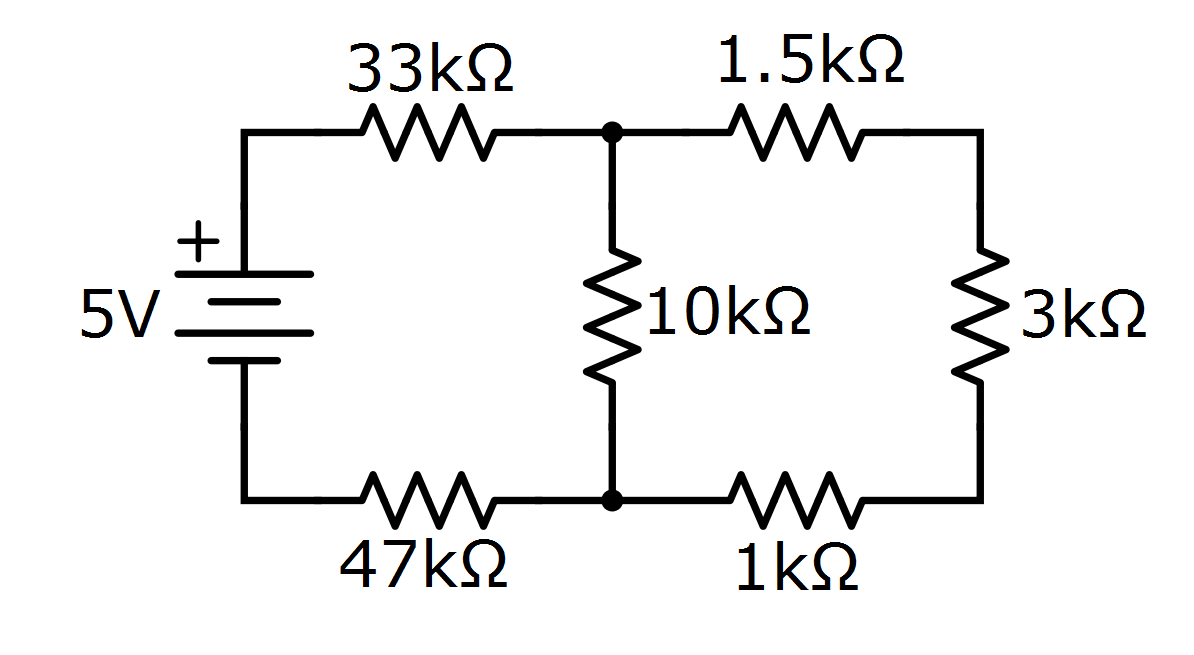
\includegraphics[width=4.65in]{figures/nodeVoltageExCircuit.png}
\caption{A circuit with several resistors.}
\label{nodeVoltageExCircuit}
\end{figure}
This circuit has 6 nodes. Each of those nodes has its own voltage. We don't know their values yet, but let's define those \textbf{node voltages} as $V_a$ through $V_f$ as shown in Figure \ref{nodeVoltageExCircuit_nodeVsAnnotated}. Also, we'll choose node ``d'' as our ground node for the circuit, making its voltage 0V.
\begin{figure}[h!]
\centering
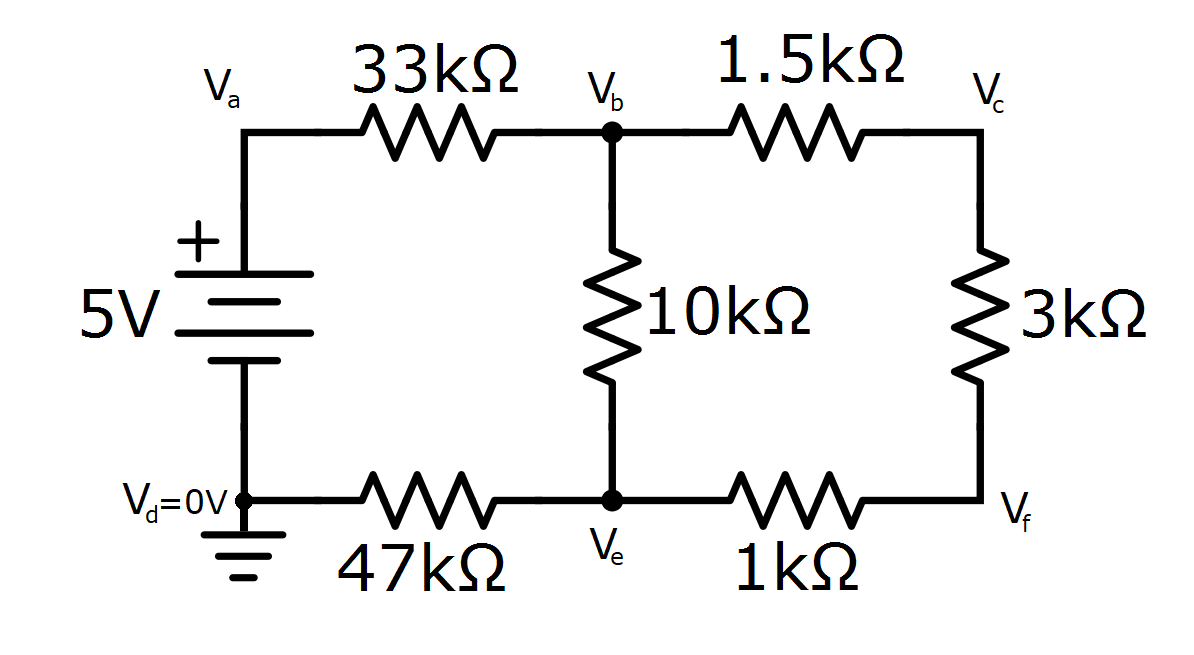
\includegraphics[width=4.65in]{figures/nodeVoltageExCircuit_nodeVsAnnotated.png}
\caption{A circuit with several resistors. Its nodes have been labeled $V_a$ through $V_f$. Additionally, we will treat $V_d$ as the circuit ground, which means we will define that node voltage as 0V.}
\label{nodeVoltageExCircuit_nodeVsAnnotated}
\end{figure}
\par
Okay, what do we do with these node voltages? Well, we need to create some equations that describe the relationships between these voltages in the circuit. We have identified six unknown node voltages, and we therefore need six unique equations to determine each of their values. Two of these equations are trivial to define---namely, $V_d=0$V and $V_a=5$V (because there is a 5V supply between $V_d$ and $V_a$). To construct the remaining four equations that relate the remaining node voltages, we will use Kirchhoff's Current Law. 
\par
Stick with me here: remember that KCL is an expression of conservation of current; at any node, the current going in is equal to the current going out. Also, the current flowing through an element can be defined as the voltage across that element divided by that element's resistance, according to Ohm's Law. 
\begin{figure}[h!]
\centering
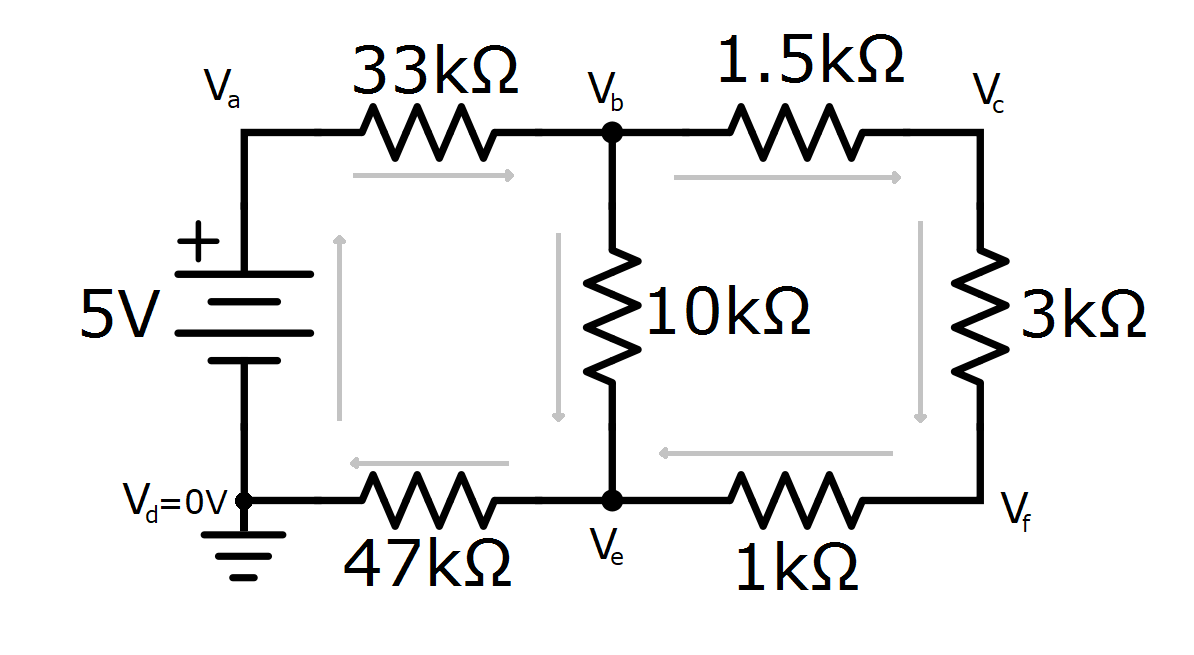
\includegraphics[width=4.65in]{figures/nodeVoltageExCircuit_nodeVsAnnotatedCurrentsDrawn.png}
\caption{The same circuit as before, but with arrows drawn to denote the direction of current flow.}
\label{nodeVoltageExCircuit_nodeVsAnnotatedCurrentsDrawn}
\end{figure}
In Figure \ref{nodeVoltageExCircuit_nodeVsAnnotatedCurrentsDrawn}, I have drawn arrows to indicate a direction for current flow in each branch. These arrows are really just guesses; it doesn't matter if I guessed correctly. All that matters is that when I create equations involving those currents, I conform to consistent assumptions. So, when I write equations to solve for the node voltages, I will adhere to my assumed current directions in Fig.~\ref{nodeVoltageExCircuit_nodeVsAnnotatedCurrentsDrawn}. 
\par
Without further ado, here we go! I'll define equations at nodes of our circuit using KCL until we have four, and then we'll construct our matrix. At node b, the current coming in can be defined as
$\frac{V_a-V_b}{33\textnormal{k}\Omega}$, while the currents leaving are $\frac{V_b-V_e}{10\textnormal{k}\Omega}$ and $\frac{V_b-V_c}{1.5\textnormal{k}\Omega}$. The equation for current at node b is therefore
$$
\frac{V_a-V_b}{33\textnormal{k}\Omega} = \frac{V_b-V_e}{10\textnormal{k}\Omega} + \frac{V_b-V_c}{1.5\textnormal{k}\Omega}
$$
\par
Moving over to node c, we see there is only one current flowing in and one current flowing out. Therefore, these currents are equal, and the KCL equation at node c is
$$
\frac{V_b-V_c}{1.5\textnormal{k}\Omega}=\frac{V_c-V_f}{3\textnormal{k}\Omega}
$$
\par
Two equations down, and two to go! It's not really possible for us to define an equation in this way at node d, because we can't define the current flowing through the 5V source in terms of node voltages. Instead, let's move on to node e. The currents at this node form the KCL equation
$$
\frac{V_b-V_e}{10\textnormal{k}\Omega} + \frac{V_f-V_e}{1\textnormal{k}\Omega} = \frac{V_e-V_d}{47\textnormal{k}\Omega}
$$
\par
Our last equation will come from the currents at node f:
$$
\frac{V_c-V_f}{3\textnormal{k}\Omega}=\frac{V_f-V_e}{1\textnormal{k}\Omega}
$$
\par
Now that we have defined six equations for our six unknown node voltages, let's list them all together:
\begin{align*}
V_d&=0\textnormal{V} \\
V_a&=5\textnormal{V}
\\
\frac{V_a-V_b}{33\textnormal{k}\Omega} &= \frac{V_b-V_e}{10\textnormal{k}\Omega} + \frac{V_b-V_c}{1.5\textnormal{k}\Omega}
\\
\frac{V_b-V_c}{1.5\textnormal{k}\Omega}&=\frac{V_c-V_f}{3\textnormal{k}\Omega}
\\
\frac{V_b-V_e}{10\textnormal{k}\Omega} + \frac{V_f-V_e}{1\textnormal{k}\Omega} &= \frac{V_e-V_d}{47\textnormal{k}\Omega}
\\
\frac{V_c-V_f}{3\textnormal{k}\Omega}&=\frac{V_f-V_e}{1\textnormal{k}\Omega}
\end{align*}
You probably noticed that this system of equations doesn't look as nice as our example system from the beginning of this chapter. You're right; these equations look like garbage. We need to manipulate these equations so that they are all of the form 
$$
c_a\cdot V_a + c_b\cdot V_b + c_c\cdot V_c + c_d\cdot V_d + c_e\cdot V_e + c_f\cdot V_f = C
$$
where all the ``c'' terms and ``C'' are constants. We can do this with just a little bit of algebraic manipulation. Ultimately, our system becomes
\begin{align*}
1\cdot V_d &= 0\textnormal{V} 
\\
1\cdot V_a &= 5\textnormal{V} 
\\
\left(\frac{1}{33\textnormal{k}\Omega}\right)\cdot V_a - \left(\frac{1}{10\textnormal{k}\Omega}+\frac{1}{1.5\textnormal{k}\Omega}+\frac{1}{33\textnormal{k}\Omega}\right)\cdot V_b +\left(\frac{1}{1.5\textnormal{k}\Omega}\right)\cdot V_c +\left(\frac{1}{10\textnormal{k}\Omega}\right)\cdot V_e &= 0\textnormal{A} 
\\
\left(\frac{1}{1.5\textnormal{k}\Omega}\right)\cdot V_b -\left(\frac{1}{1.5\textnormal{k}\Omega}+\frac{1}{3\textnormal{k}\Omega}\right)\cdot V_c + \left(\frac{1}{3\textnormal{k}\Omega}\right)\cdot V_f &= 0\textnormal{A} 
\\
\left(\frac{1}{10\textnormal{k}\Omega}\right)\cdot V_b +\left(\frac{1}{47\textnormal{k}\Omega}\right)\cdot V_d -\left(\frac{1}{1\textnormal{k}\Omega}+\frac{1}{10\textnormal{k}\Omega}+\frac{1}{47\textnormal{k}\Omega}\right)\cdot V_e +\left(\frac{1}{1\textnormal{k}\Omega}\right)\cdot V_f &= 0\textnormal{A} 
\\
\left(\frac{1}{3\textnormal{k}\Omega}\right) \cdot V_c + \left(\frac{1}{1\textnormal{k}\Omega}\right)\cdot V_e -\left(\frac{1}{1\textnormal{k}\Omega}+\frac{1}{3\textnormal{k}\Omega}\right)\cdot V_f &= 0\textnormal{A}
\end{align*}
from which we can extract the matrix:
$$
\begin{bmatrix}
    0 & 0 & 0 & 1 & 0 & 0 & 0 \\
    1 & 0 & 0 & 0 & 0 & 0 & 5 \\
	(1/33) & -(263/330) & (2/3) & 0 & (1/10) & 0 & 0 \\
	0 & (2/3) & -1 & 0 & 0 & (1/3) & 0 \\
	0 & (1/10) & 0 & (1/47) & -(527/470) & 1 & 0 \\
	0 & 0 & (1/3) & 0 & 1 & -(4/3) & 0
\end{bmatrix} 
$$
Notice that I removed the units from all the coefficients before I put them into the matrix. I also found common denominators for all the summed fractions so that the coefficients could remain in fractional form.
\par
Using a computer to find the RREF for the above matrix yields:
$$
\begin{bmatrix}
    1 & 0 & 0 & 0 & 0 & 0 & 5 \\
    0 & 1 & 0 & 0 & 0 & 0 & 3.03 \\
	0 & 0 & 1 & 0 & 0 & 0 & 2.97 \\
	0 & 0 & 0 & 1 & 0 & 0 & 0 \\
	0 & 0 & 0 & 0 & 1 & 0 & 2.81 \\
	0 & 0 & 0 & 0 & 0 & 1 & 2.85 \\
\end{bmatrix} 
$$
We now know the values of all of the node voltages in our original circuit, as shown in Figure~\ref{nodeVCircuit_VsLabeled}.
%\begin{align*}
%V_a &= 5\textnormal{V} \\
%V_b &= 3.03\textnormal{V} \\
%V_c &= 2.97\textnormal{V} \\
%V_d &= 0\textnormal{V} \\
%V_e &= 2.81\textnormal{V} \\
%V_f &= 2.85\textnormal{V} 
%\end{align*}
\begin{figure}[h!]
\centering
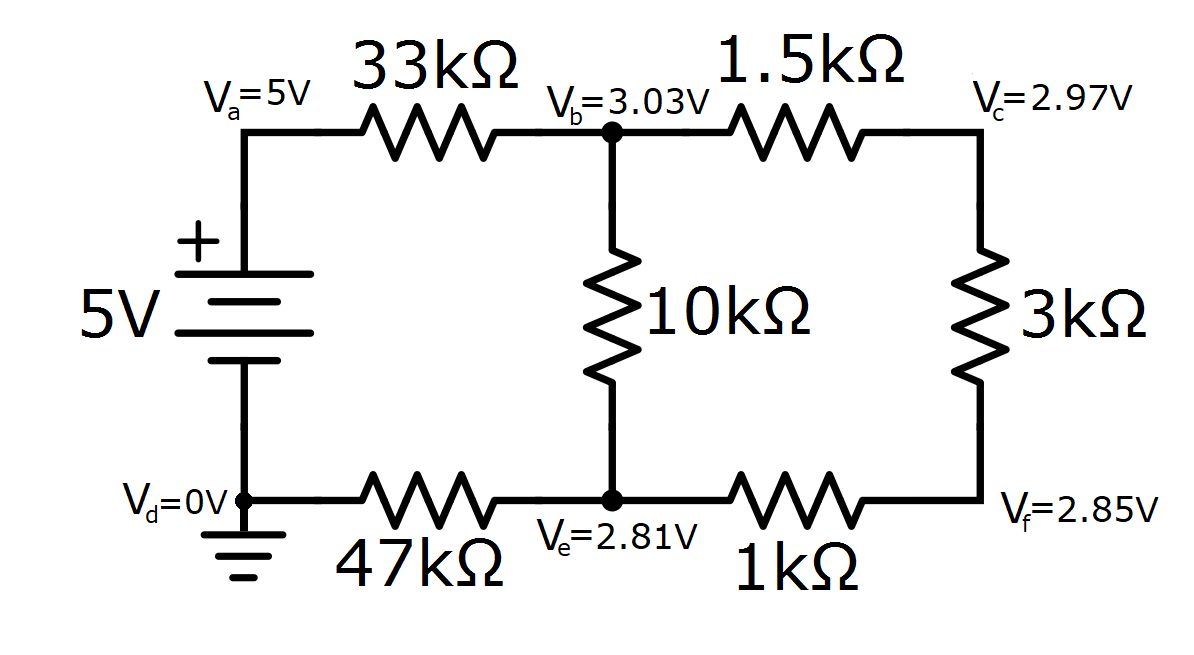
\includegraphics[width=4.65in]{figures/nodeVoltageExCircuit_nodeVnumbers.png}
\caption{The same circuit as before, but with node voltages labeled.}
\label{nodeVCircuit_VsLabeled}
\end{figure}
\par
After performing node voltage analysis on a circuit, we have enough information to determine the current flowing through or the power dissipated by any element in the circuit, and we didn't have to mangle the original circuit (like we would have if we had found a Norton or Thevenin equivalent). Sometimes, however, node voltage analysis can be more cumbersome than it is worth. The mesh current analysis technique can also be used to analyze an entire circuit at once, and in some situations it can be simpler to execute. We'll explore this technique in the next section.
\section{Mesh Current Analysis}
To use the mesh current analysis technique, we must first determine how many \textit{meshes} there are in our circuit of interest. A mesh is a loop in a circuit that doesn't encircle any other loops. To demonstrate mesh current analysis, we will use the same circuit as we did in the node voltage analysis section. That circuit has two meshes, and it is displayed again in Figure \ref{meshCurrentCircuit}.
\begin{figure}[h!]
\centering
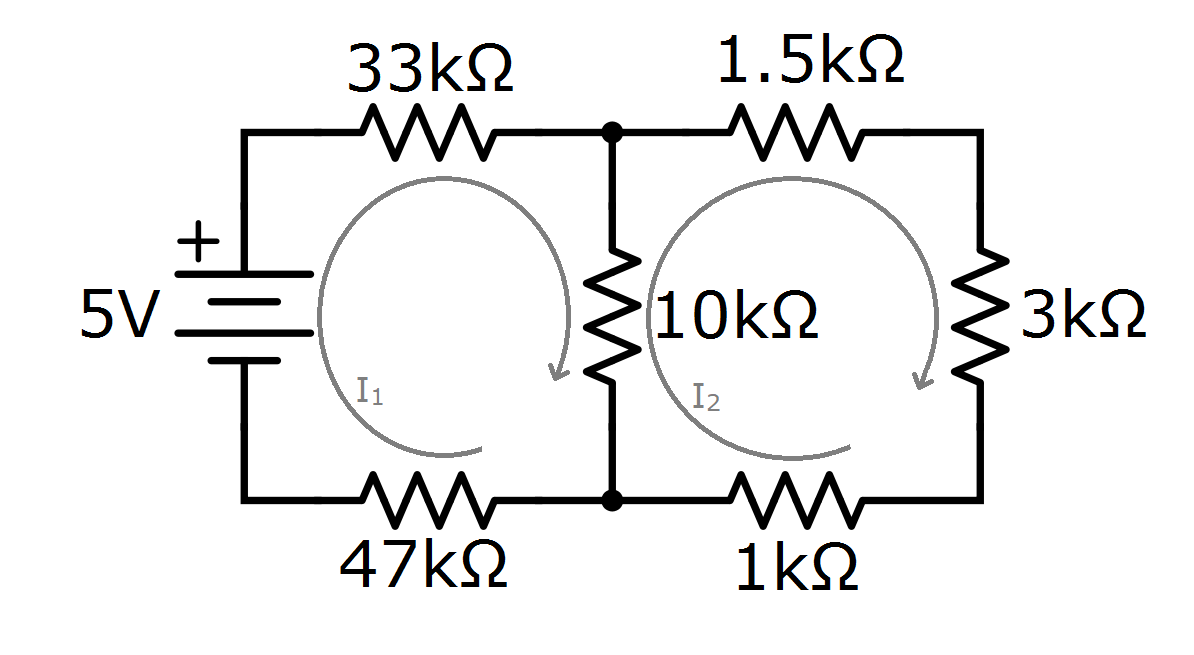
\includegraphics[width=4.65in]{figures/meshCurrentExCircuit.png}
\caption{A circuit we will analyze using the mesh current analysis technique. The two mesh currents for this circuit are already drawn on the schematic.}
\label{meshCurrentCircuit}
\end{figure}
In each of the two meshes of this circuit, I have drawn a circular-looking current. These currents are called \textit{mesh currents}, because each one flows around a single mesh in the circuit. When only one mesh current flows through an element, it behaves just like the branch currents we have already seen. However, when there are two mesh currents flowing through an element, those mesh currents add up to make a single branch current. For example, the branch current flowing from top to bottom through the 10k$\Omega$ resistor in the middle of the circuit can be written in terms of the mesh currents as $I_1-I_2$.
\par
To fully analyze the circuit of Figure~\ref{meshCurrentCircuit}, we need to determine the values of its two unknown mesh currents. To do that, we need to create a system of two equations (because we have two unknown quantities) to describe the circuit in terms of the mesh currents. We will use KVL to create these equations as follows.
\par
To create equations, I like to focus on one mesh at a time, accounting for the voltages added and dropped as I trace through all the elements in the mesh. If we focus on mesh 1 in the example circuit, we can create the following equation: 
$$
5\textnormal{V} - I_1\cdot33\textnormal{k}\Omega -(I_1-I_2) \cdot 10\textnormal{k}\Omega - I_1\cdot47\textnormal{k}\Omega = 0\textnormal{V}
$$
Notice that, when I accounted for the voltage drop across the $10\textnormal{k}\Omega$ resistor, I combined the two mesh currents by subtracting $I_2$ from $I_1$. I did this because the current flowing in the downward direction through that resistor is a combination of both mesh currents, and the two mesh currents actually work against each other because they are flowing in opposite directions through that resistor. I could have alternatively accounted for both voltages separately by subtracting $I_1\cdot10\textnormal{k}\Omega$ and adding $I_2\cdot10\textnormal{k}\Omega$. In general, I prefer to combine mesh currents and write a term with that combined current, but you can do what feels right to you.
\par
By accounting for the voltages added and dropped in mesh 2, we can create the following equation:
$$
-(I_2-I_1) \cdot 10\textnormal{k}\Omega - I_2\cdot1.5\textnormal{k}\Omega - I_2\cdot3\textnormal{k}\Omega - I_2\cdot1\textnormal{k}\Omega = 0\textnormal{V}
$$
Now that we have two equations, we can solve this system of equations to find the values for the two unknown mesh currents in our circuit. First, we need to rearrange the equations to consolidate all of the $I_1$ terms and $I_2$ terms in each equation as follows:
\begin{align*}
90\textnormal{k}\Omega \cdot I_1 - 10\textnormal{k}\Omega \cdot I_2 &= 5\textnormal{V} \\
10\textnormal{k}\Omega \cdot I_1 - 15.5\textnormal{k}\Omega \cdot I_2 &= 0\textnormal{V}
\end{align*}
From these equations, we can extract the matrix
$$
\begin{bmatrix}
90000 & -10000 & 5 \\
10000 & -15500 & 0
\end{bmatrix}
$$
For which the RREF is 
$$
\begin{bmatrix}
1 & 0 & 0.00006 \\
0 & 1 & 0.00004
\end{bmatrix}
$$
Therefore, the mesh currents in this circuit are
\begin{align*}
I_1&=0.06\textnormal{mA} \\
I_2&=0.04\textnormal{mA}
\end{align*}
I can use these mesh currents to find node voltages. For example, assuming the bottom-left node in the circuit is the ground node, I know that the voltage of the top middle node is $5\textnormal{V}-I_1\cdot33\textnormal{k}\Omega = 5\textnormal{V}-(0.06\cdot33)\textnormal{V} = 3.03\textnormal{V}$ with respect to ground. Notice that this is the same voltage as we found for $V_b$ when we used the node voltage method to solve this circuit. 

\section{Recap}
The two analysis techniques described in this chapter are not only useful for DC resistive circuits; they can also be used to analyze AC circuits with inductors and capacitors. Once you get used to the process of constructing the matrices involved, these techniques allow you to quickly analyze an entire circuit.
\begin{description}
\item[Node Voltage Analysis] This technique involves the use of Kirchhoff's Current Law to find the voltage at each node in a circuit. The following steps must be taken to apply the node voltage analysis method:
\begin{enumerate}
\item Identify and label all nodes
\item Choose a ground node, and assign that node voltage to be 0V
\item Draw currents in the circuit
\item Use Ohm's Law to define the currents you drew in terms of node voltages and resistances
\item Use KCL to write equations at the nodes; you need as many equations as you have unknown currents
\item Rearrange each of your equations so that you can create a matrix with the coefficients of the node voltages in your system of equations
\item Use a computer to find the RREF of the matrix; the right-most column in the resulting matrix will hold the values for all the node voltages in the circuit
\end{enumerate}

\item[Mesh Current Analysis] This technique involves the use of Kirchhoff's Voltage Law to find the values for mesh currents in a circuit. The following steps define the mesh current method:
\begin{enumerate}
\item Draw and label mesh currents in each mesh of the circuit
\item Use KVL to write equations around each mesh in the circuit
\item Rearrange each of your equations so that you can create a matrix with the coefficients of the mesh currents in your system of equations
\item Use a computer to find the RREF of the matrix; the right-most column in the resulting matrix will hold the values for all the mesh currents in the circuit
\end{enumerate}
\end{description}
